\documentclass{capstonedoc}

% Document Info
\title{Sega Genesis Controller Interfacing}
\date{2016-01-23}
\author{Stephen Just}

\usepackage{cite}
\usepackage[hyphens]{url}
\usepackage{graphicx}
\graphicspath{ {images/} }

\begin{document}
\maketitle

%Document body

\section{Introduction}
The Sega Genesis was an old 16-bit game console that was released in North
America in 1989. \cite{SGHistory}

This console features support for two gamepads. Each gamepad has four
directional buttons, a ``Start'' button, and either three or six action
buttons, depending on model of controller. The three-button controller has a
much simpler interface than the six-button controller, making use of a
multiplexer and no other logic to access all of the buttons. This document
focuses only on the three-button Genesis controller. The Genesis controllers
also use a standard DB-9 connector, unlike most other game consoles which
use proprietary connectors.\cite{SGCHwInfo}

\section{Controller Interface}
The Genesis controller uses a female DB-9 connector to interface with a Genesis
console or other device. The pins on this connector are configured as follows:

\vspace{5mm}
\begin{tabular}{ l | l | l }
  Pin & Func (select low) & Func (select high) \\ \hline \hline
  1   & up button         & up button          \\
  2   & down button       & down button        \\
  3   & logic low         & left button        \\
  4   & logic low         & right button       \\
  5   & Power (+5 volts)  & Power (+5 Volts)   \\
  6   & A button          & B button           \\
  7   & select signal     & select signal      \\
  8   & Ground            & Ground             \\
  9   & Start button      & C button           \\
\end{tabular}
\vspace{5mm}

\begin{figure}[t]
  \centering
  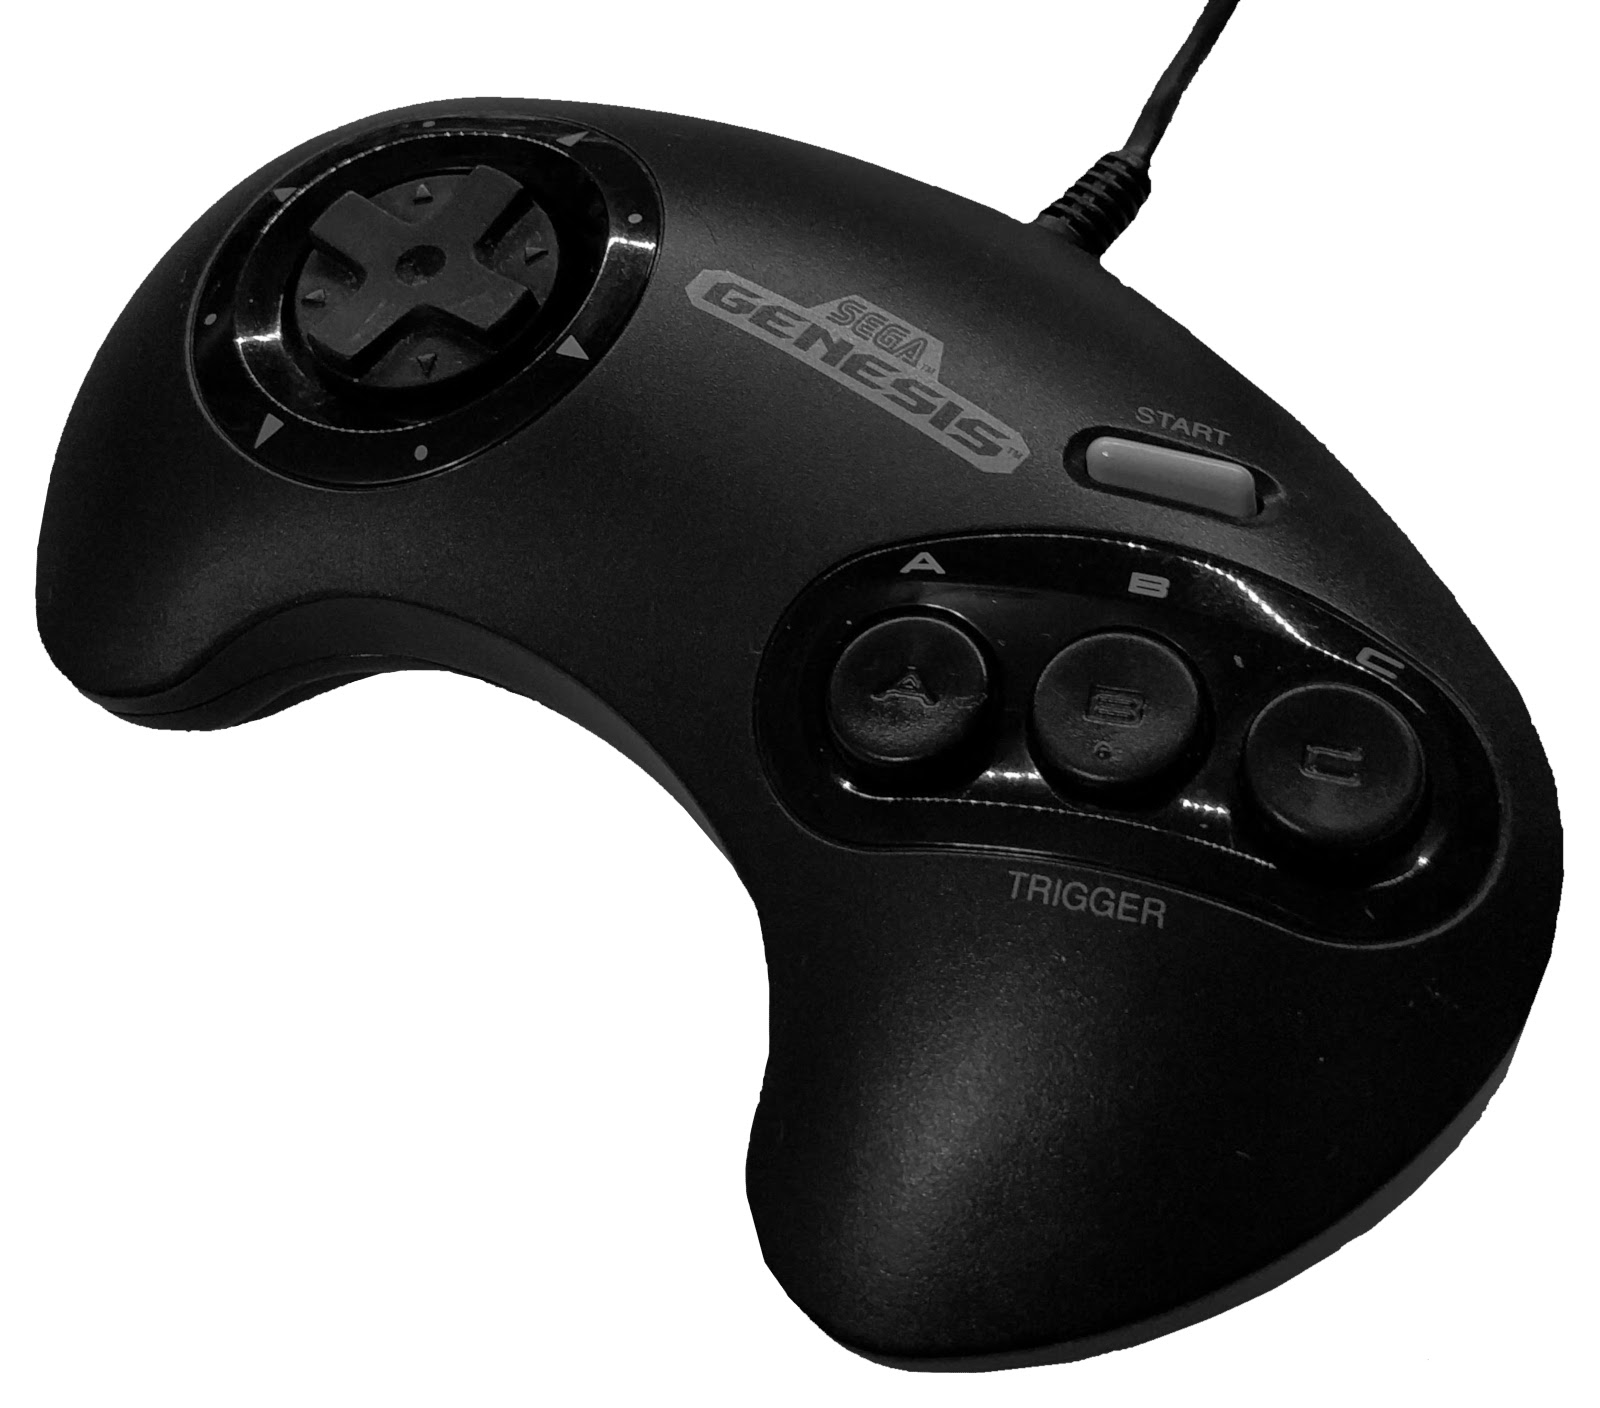
\includegraphics[width=6cm]{genesis_controller}
\end{figure}

While the controller was designed for +5 Volts for power, because of its simple
design, it is possible to determine that it is actually capable of 2 - 6 Volts.
This is possible because the controller only contains a single 74HC157
multiplexer chip inside, whose datasheet specifies that the device is operable
within that range, with varying delay times.\cite{TC74HC157AP}

In order to read the buttons on a controller, the master device should apply
a logic high or low to the select pin of the controller, and then query the
state of each of the button pins. Then the master device can switch the state
of the select pin, and then query the values for the other buttons. When a
button is pressed, its value will be logic low. Buttons that are not pressed
will appear as a logic high. Note that reading the up and down buttons of
the controller are not affected by the select signal, as they are connected
directly to the controller plug and not through the multiplexer.

\section{Notes}
On a real Genesis console, the controller's value is read once per video frame,
or 60 times per second. That means that if you are trying to emulate a
controller, the emulated buttons should remain pressed for at least 1/60th of
a second, to ensure that the input is received by the console. Shorter button
presses could be missed entirely.

Be aware that the six-button gamepad has a more complicated interface protocol.
The extra buttons are accessed by toggling the select line on the controller
three times in quick succession. If you want your application to tolerate six-
button controllers, take care not to do this. The six-button controllers should
not go in to this mode if you only toggle the select line once per frame.

\begin{lstlisting}[language={vhdl},float]
-- A comment
\end{lstlisting}

% References
\bibliographystyle{ieeetr}
\bibliography{genesis_controller}

\end{document}
